\chapter{Konzeption}
\label{ch:konzeption}
In diesem Kapitel wird die grundlegende Konzeption der Arbeit vorgestellt.

\section{Methodisches Vorgehen}
Es soll eine Beispielanwendung sowohl in containerisierter Form als auch Serverless entwickelt werden. Die Konzeption dieser beiden Anwendungen wird in den folgenden Abschnitten genauer beschrieben. 
Im Anschluss werden Performance-Tests beider Anwendungen durchgeführt und die Ergebnisse miteinander verglichen. Die Forschungsfrage wurde dazu in kleinere Teilfragen (Research-Questions \hyperref[tab:research-questions]{RQ1} bis \hyperref[tab:research-questions]{RQ5}) aufgeteilt, die im Laufe der Analyse untersucht werden sollen und unterschiedliche Performance Aspekte betrachten. Die Fragen sind in Tabelle \ref{tab:research-questions} aufgelistet.

\begin{table}[H]
\begin{tabularx}{\textwidth}{|l|X|}
\hline
RQ1 & Wie viel Last kann eine einzige Container-Instanz tragen und wie vielen nebenläufigen Lambda-Funktionen entspricht dies? \\ \hline
RQ2 & Wie unterscheidet sich die Performance bei normaler und schnell ansteigender Last?                                                          \\ \hline
RQ3 & Welchen Einfluss hat die Nutzung größerer CPU / RAM Werte?                                                              \\ \hline
RQ4 & Welchen Einfluss hat die Nutzung mehrerer Container-Instanzen auf die Performance?                                      \\ \hline
RQ5 & Welchen Einfluss haben die unterschiedlichen Use-Cases auf die Performance?                                                  \\ \hline
\end{tabularx}
\caption{\label{tab:research-questions}Research-Questions dieser Arbeit}
\end{table}

Das methodische Vorgehen für den Aufbau der Test-Umgebung basiert dabei grundlegend auf den von Papadopoulos et. al. vorgestellten methodologischen Prinzipien für reproduzierbare Performance-Evaluation im Cloud Computing Umfeld, die in Tabelle \ref{tab:principles} beschrieben werden\cite{papadopoulos_methodological_2019}.

Das Prinzip \hyperref[tab:research-questions]{P4} wird erfüllt durch die Nutzung eines öffentlichen GitHub Repositories unter \url{https://github.com/rolule/ba}, in dem sowohl die Skripte die zur Generierung der Tests verwendet wurden, als auch die Output-Artefakte der Tests abgelegt sind (siehe Anhang \ref{apx:repo}).

Im Anschluss an die Performance-Tests wird auf die Kostenmodelle der beiden Technologien eingegangen.

\begin{table}[H]
\begin{tabularx}{\textwidth}{|l|X|}
\hline
P1 & Wiederholte Durchführung (Repeated experiments): Mehrere Experimente mit der selben Konfiguration durchführen. In dieser Arbeit wird jeder Test mindestens zwei mal durchgeführt, um einmalige Aussetzer erkennen zu können. \\ \hline

P2 & Konfigurations-Abdeckung (Workload and configuration coverage): Experimente in verschiedenen Konfigurationen der relevanten Parameter durchführen. Beispielsweise verschiedene Hardware-Konfigurationen aber auch verschiedene Load-Testing-Typen (z.B. Spike-Test). \\ \hline

P3 & Experimenteller Aufbau (Experimental setup description): Beschreibung der Hardware- und Software (inklusive Version), und anderer Parameter die für das Experiment genutzt wurden und einen Einfluss auf dessen Ausgang haben können. Zusätzlich sollte die Beschreibung das genaue Ziel des Experiments beinhalten. \\ \hline

P4 & Offener Zugang zu Artefakten (Open access artifact): Möglichst viele für die Experimente genutzten Konfigurationsdateien, Protokolle, etc. sollten versioniert und offen zugänglich sein. \\ \hline

P5 & Probabilistische Ergebnisbeschreibung der gemessenen Performance (Probabilistic result description of measured performance): Angemessenes Beschreiben und Visualisieren der Ergebnisse. Verwendung von Quantilen (z.B. Median oder 95. Quantil) und der Standardabweichung. \\ \hline

P6 & Statistische Auswertung: Statistische Tests anwenden, um die Validität der Studie zu untermauern. Dieses Prinzip wird aus mangelnder Expertise nicht genauer betrachtet, daher hier der Hinweis, dass die Ergebnisse dieser Arbeit eventuell nicht signifikant sein könnten. \\ \hline

P7 & Einheiten (Measurement units): Für alle Messungen die zugehörigen Einheiten angeben. \\ \hline

P8 & Kosten (Cost): Kostenmodell, Ressourcennutzung und abgerechnete Kosten angeben. \\ \hline
\end{tabularx}
\caption{\label{tab:principles}Prinzipien für reproduzierbare Performance-Evaluation im Cloud-Computing Umfeld nach Papadopoulos et. al.\cite{papadopoulos_methodological_2019}}
\end{table}

\section{Konzeption der Test-Anwendungen}
Als Testanwendung wird ein einfaches HTTP-REST-Backend am Beispiel einer Notiz-Applikation entwickelt. Der Service stellt folgende Routen bereit:  

\begin{enumerate}
    \item GET /notes: Das Auflisten aller verfügbarer Notizen
    \item GET /notes/\{id\}: Das Auflisten eines spezifischen Notiz mit der angegebenen id
    \item PUT /notes/\{id\}: Das Ändern einer spezifischen Notiz mit der angegebenen id
    \item POST /: Das Erstellen einer Notiz
\end{enumerate}

Um die Anwendung möglichst einfach zu gestalten und Unterschiede zwischen den beiden Technologien zu minimieren, wird auf die Verwendung einer Datenbank verzichtet. Stattdessen wird ein Delay von 50 Millisekunden für jeden Request eingebaut. 
Auch auf Authorisierungs-Mechanismen wird der Einfachheit halber verzichtet. Dies erlaubt es außerdem, von einer konstanten Benutzer-Rate auszugehen, da alle "`eingeloggten"' Benutzer auch gleichzeitig aktiv sind\cite{molyneaux_art_2014}. 
Als Runtime wird sowohl bei der Serverless- als auch bei der containerisierten Anwendung Node.js 12 verwendet.

\subsection{Serverless}
Für die Entwicklung der Serverless-Anwendung wird das mit mehr als \linebreak 38.000 Github-Stars populäre Serverless-Framework in der Version 2.21.0 verwendet\cite{noauthor_serverlessserverless_nodate}. Dabei handelt es sich um ein Open-Source Framework zur Entwicklung von Serverless-Anwendungen. Es übernimmt die Erstellung von Anwendungs-Stacks, Rechteverteilung und Konfiguration bei allen gängigen Public-Cloud Anbietern wie \ac{AWS}, Microsoft Azure oder \ac{GCP}. Da in dieser Arbeit \ac{AWS} verwendet wird, erstellt Serverless automatisch einen Anwendungs-Stack mit \ac{AWS} CloudFormation. 
Abbildung \ref{fig:serverless-testing-architektur} zeigt das Setup der mit der Serverless-Architektur konzipierten Webanwendung.

\begin{figure}[H]
    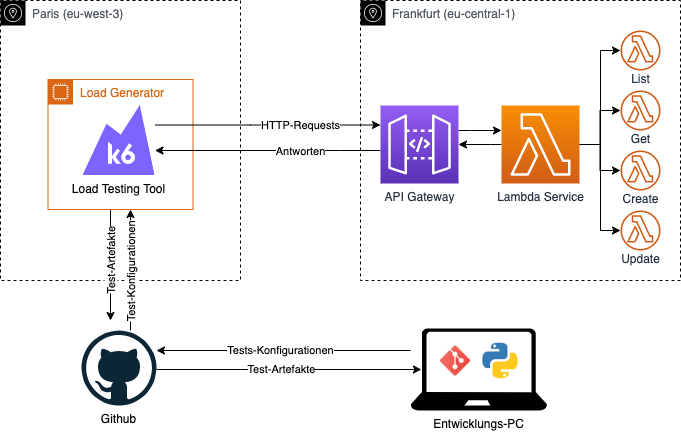
\includegraphics[width=\textwidth]{img/serverless-testing-architektur.png}
    \caption[Testing-Architektur der Serverless Notiz-Anwendung]{Testing-Architektur der Serverless Notiz-Anwendung}
    \label{fig:serverless-testing-architektur}
\end{figure}

Der vom Serverless-Framework bzw. CloudFormation erstellte \linebreak Anwendungs-Stack beinhaltet ein Amazon API-Gateway, das über die Routen der REST-Schnittstelle verfügt. Trifft eine HTTP-Anfrage des Load-\linebreak Generators an eine der Routen ein, übernimmt das API-Gateway die Auslösung des passenden Events, wodurch der Lambda-Service die korrekte Lambda-Funktion startet und mit den im HTTP-Request übergebenen Parametern aufruft. Nach Beendigung der Funktion wird ihr Rückgabewert über das API-Gateway zurück an den Load-Generator gesendet. Jeder Start einer Lambda-Funktion erfordert das Herunterladen des Codes, der in der Funktion ausgeführt werden soll. Dazu wird der Code vom Serverless-Framework in einen \ac{S3}-Bucket hochgeladen und bei Bedarf vom Lambda-Service angefordert (vgl. Abbildung \ref{fig:lambda-architecture}).

Durch die Nutzung des Frameworks wird die Erstellung der Anwendung vereinfacht. Die Konfiguration des API-Gateways und des \ac{S3}-Buckets werden automatisch erledigt. In Zukunft kann die Analyse durch Nutzung des Frameworks leicht auf \ac{FaaS}-Angebote weiterer Cloud-Anbieter wie Microsoft Azure Functions oder Google Cloud Functions erweitert werden.

\subsection{Container}
Für die Entwicklung der containerisierten Anwendung wird das Express-Framework in der Version 4.17.1 verwendet, das mit über 51.000 Github-Stars ein weit verbreitetes Web-Frameworks für Node.js ist\cite{noauthor_expressjsexpress_2021}. Die Anwendung wird unter Nutzung der Docker-Engine (Version 20.10.0) mittels einer Dockerfile in ein Container-Image gebaut. Dieses Image wird in der \ac{AWS} Elastic Container Registry (ECR) gespeichert, um es von dort aus weiter zu verwenden. 
Die Ausführung der Anwendung erfolgt auf \ac{ECS}, einem von \ac{AWS} bereitgestelltem Orchestrations-Tool. Es wird der Starttyp Fargate benutzt, welcher die Erstellung und Verwaltung eines Server-Clusters automatisch übernimmt und so die Konfiguration erleichtert. Des Weiteren wird ein \ac{ELB} vom Typ Application verwendet, um die eingehenden Requests auf die verschiedenen Container zu verteilen. 

Abbildung \ref{fig:fargate-testing-architektur} zeigt das Setup der mit der Container-Architektur konzipierten Notiz-Anwendung. Bei der Konfiguration des Container-Clusters muss für Fargate eine Task-Definition erstellt werden. Diese definiert alle Tasks die gleichzeitig in einem Service laufen sollen. Ein Service konfiguriert die Ausführung mehrerer Container-Instanzen. In dieser Arbeit wird, außer bei den Tests mit mehreren Instanzen, für jeden Service nur ein einziger Task, also eine einzige Container-Instanz jedem Service zugeordnet. \ac{ECS} erlaubt nur bestimmte Paare von CPU und Arbeitsspeicher-Einstellungen für einen Container. Für die Tests mit 128MB und 256MB Speicher wird das Einstellungs-Paar mit 512MB RAM und 0.25 vCPU festgelegt und die einzelnen Container mit entsprechenden harten Limits von 128MB und 256MB für den Arbeitsspeicher konfiguriert. Für die Tests mit 512MB wird die Einstellungs-Paar mit 1GB RAM und 0.5 vCPU verwendet, der ein hartes Limit von 512MB Speicher zugewiesen bekommt. Ein \ac{vCPU} beschreibt laut \ac{AWS} hierbei einen Thread eines CPU-Kerns\cite{noauthor_cpu-optionen_nodate}. Die verwendeten Task-Definitionen sind in Anhang \ref{apx:task-definitions} aufgelistet. Sie werden mittels der \ac{AWS} Konsole erstellt und konfiguriert.

\begin{figure}
    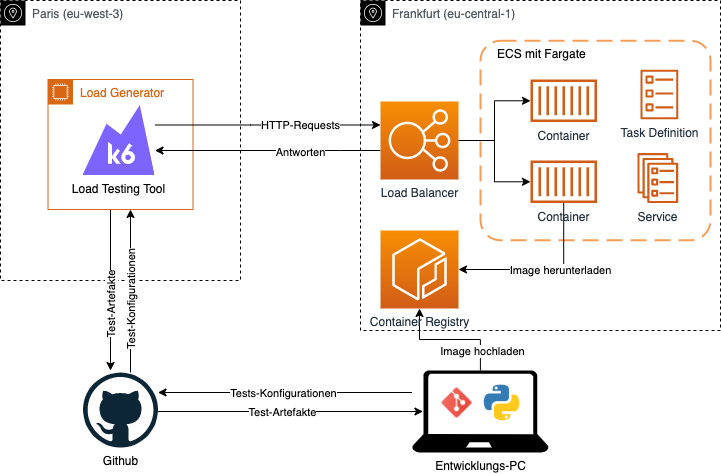
\includegraphics[width=\textwidth]{img/fargate-testing-architektur.png}
    \caption[Testing-Architektur der Container Notiz-Anwendung]{Testing-Architektur der Container Notiz-Anwendung}
    \label{fig:fargate-testing-architektur}
\end{figure}

\section{Konzeption der Tests}

\subsection{Testing-Tool}
Um die Performance der eben vorgestellten Anwendungen zu testen, wird das Open-Source Performance-Testing-Tool k6 \cite{noauthor_load_nodate} verwendet. Durch eine optimierte CPU-Auslastung ermöglicht es, ohne die Notwendigkeit einer verteilten Ausführung, etliche virtuelle Benutzer zum Testen einer Anwendung zu kreieren\cite{noauthor_running_nodate}. Die Benutzer arbeiten parallel die in Sektion \ref{sec:use-cases} vorgestellten Use-Cases ab, bei denen verschiedene Anfragen an die REST-APIs der Services geschickt werden. Die Abläufe der Anwendungsfälle werden dafür in der von k6 unterstützten Skripting-Sprache JavaScript geschrieben und dem Tool bei der Ausführung übergeben.

Als Load-Generator wird eine in der \ac{AWS} Region Paris (eu-west-3) stationierte \ac{EC2} Instanz des Typs t3.xlarge verwendet.
Nach eigenen Angaben benötigt k6 für jeden virtuellen Benutzer und für einen kleinen Test eine Speicherauslastung zwischen 1 und 5 Megabyte\cite{noauthor_running_nodate}. Da die verwendete t3.xlarge Instanz 16 Gigabyte RAM beinhaltet, sollten theoretisch mehr als 3.200 und maximal 16.000 gleichzeitige virtuelle Benutzer von der Testumgebung unterstützt werden. Die Instanz weist eine Netzwerkleistung von bis zu 5 Gbit/s auf, welche bei jeder Testausführung mittels des Tools \textit{iftop} überwacht wird, um sicherzugehen, dass das Netzwerk nicht zum Flaschenhals wird. Auch die CPU-Auslastung wird mittels \textit{htop} überprüft. Es wurde eine andere Region für den Load-Generator gewählt, um keine Ergebnisverfälschungen durch eventuell optimierte Routing-Mechanismen innerhalb eines \ac{AWS} Rechenzentrums zu verursachen.

Die Tests werden ausgeführt, indem vom Entwicklungscomputer eine SSH Verbindung zum Load-Generator aufgebaut wird. Dann wird der Test-Code über das GitHub-Repository heruntergeladen. Zur Ausführung der Tests und automatisch komprimierter Speicherung der Test-Artefakte im Repository wurde ein Node.js Skript geschrieben, welches unter dem Dateinamen "`test.js"' zu finden ist. Das Skript liest von der Kommandozeile die Parameter des aktuellen Tests ein und startet dann k6 mit dem vom Benutzer ausgewählten Test-Szenario (siehe Anhang \ref{apx:repo}). 

\subsection{Metriken}
Das Testing-Tool k6 speichert für jeden Request an einen bestimmten API-Endpunkt unter anderem Werte folgender Metriken:
\begin{enumerate}
    \item \acp{VU}: Die Anzahl der virtuellen Benutzer zum aktuellen Zeitpunkt.
    
    \item Antwortzeit (Response Time): Die Zeit vom Abschicken eines Requests bis zum Erhalt der Antwort in Millisekunden (ms). Dabei wird Aufwand für eventuelle DNS Lookups nicht mit einberechnet\cite{noauthor_metrics_nodate}. 
    
    \item HTTP-Statuscodes: Geben den Status eines HTTP-Requests an. Wichtig für die Betrachtung sind vor allem die Codes:
        \begin{enumerate}
            \item 200 (OK): Der Request war erfolgreich\cite{noauthor_200_nodate}.
            \item 500 (Internal Server Error): Der Server konnte den Request aufgrund eines nicht vorhergesehenen Problems nicht angemessen verarbeiten\cite{noauthor_500_nodate}.
            \item 502 (Bad Gateway): Der Server ist überlastet oder kann aus anderen Gründen nicht erreicht werden\cite{noauthor_error_nodate}.
            \item 503 (Service Unavailable): Der Server ist überlastet oder für Wartungsarbeiten abgeschaltet\cite{noauthor_503_nodate}.
            \item 504 (Gateway Timeout): Der als Gateway / Proxy agierende Server konnte innerhalb eines festgelegten Zeitintervalls keine Antwort liefern\cite{noauthor_http_nodate}.
        \end{enumerate}
        
    \item Request-Rate: Die durchschnittliche Anzahl der Requests pro Sekunde.
\end{enumerate}

Für Analysen und Vergleiche mehrerer Test-Ausführungen untereinander, werden die Ergebnisse jedes k6-Tests als \ac{CSV} Text-Datei exportiert. Im Anschluss können diese Dateien mit dem Data-Science Framework Pandas\cite{noauthor_pandas_nodate} für die Programmiersprache Python analysiert und verglichen werden. Der Source-Code der Analysen und die \linebreak Ergebnis-Artefakte der Tests sind im Code-Repository dieser Arbeit zu finden (vgl. Anhang \ref{apx:repo}).

Weitere Metriken wie die CPU-Auslastung eines Fargate-Clusters und die maximale Nebenläufigkeit, Funktions-Dauer und Coldstart-Dauer werden von der \ac{AWS} CloudWatch Konsole abgelesen und können daher nicht als Artefakte gespeichert werden.

\subsection{Test-Typen}
Bei Performance-Tests können verschiedene Testing-Strategien eingesetzt \linebreak werden. Die für diese Arbeit relevanten Strategien sind Load- und Stress-Tests:
\begin{enumerate}
    \item Load Testing: Dient der Evaluierung der System-Performance in Bezug auf die Anzahl der gleichzeitigen Benutzer oder der Requests-Rate. Es wird der Normalbetrieb des Systems simuliert\cite{noauthor_what_nodate-2}.
    
    \item Stress Testing: Dient dazu, die Grenzen des Systems in den Punkten Verfügbarkeit und  Stabilität auszutesten. Man geht über den normalen Betrieb hinaus und eventuell so hoch, dass das System der Last nicht mehr standhalten kann. Bei einem Stress-Test wird schrittweise die Last auf das System erhöht. So kann man zum Beispiel herausfinden, ob das System großen Anstürmen, wie z.B einem Sale-Event bei einem Online-Shop, Stand halten kann\cite{noauthor_what_nodate-1}.
\end{enumerate}

Es gibt noch weitere Test-Typen wie Smoke- oder Soak-Tests, die allerdings keine Relevanz für die Zielfragen dieser Arbeit haben und daher nicht betrachtet werden.

\subsection{Getestete Use-Cases}\label{sec:use-cases}
Die folgenden Use-Cases werden bei der Analyse der \acp{SUT} evaluiert. 
In der Aufzählung ist immer zuerst das verwendete HTTP-Verb (GET, POST, PUT) und danach der korrespondierende Endpunkt der Applikation aufgelistet. Die nach dem Pfeil angegebenen Zeitintervalle entsprechen der sogenannten "`Think Time"', also der Zeit die ein Benutzer normalerweise benötigt um sich für seine nächste Handlung zu entscheiden. Es wird, wie von Molyneaux empfohlen, mit einer ±10 prozentigen Abweichung versucht, eine realistischere Szenariodurchführung zu erreichen\cite{molyneaux_art_2014}. Um möglichst realitätsnahe Ergebnisse zu erzielen, wird davon ausgegangen, dass der Benutzer etwa eine Sekunde benötigt, um sich einen Überblick über alle Notizen zu verschaffen oder einen Fehler in der Notiz zu erkennen und etwa drei Sekunden, um eine Notiz zu erstellen oder zu bearbeiten. Am Ende jedes Use-Cases wird zudem eine Wartezeit von etwa einer Sekunde eingefügt, um den darauf folgenden ersten Request der nächsten Iteration nicht sofort nach dem letzten Request der aktuellen Iteration durchzuführen. 
\begin{itemize}
    \item Use-Case A: Alle Notizen abrufen \\
        Alle Notizen einmal abrufen. \\
        1. GET /notes $\rightarrow$ 1s     \\

    \item Use-Case B: Notiz bearbeiten \\
        Erst alle Notizen, dann eine einzelne Notiz abrufen und bearbeiten. \\
        1. GET /notes $\rightarrow$ 1s     \\
        2. GET /notes/1 $\rightarrow$ 3s   \\
        3. PUT /notes/1 $\rightarrow$ 1s   \\
        
    \item Use-Case C: Notiz falsch erstellt \\
    Der Benutzer ruft alle Notizen ab. Er entscheidet sich eine Notiz zu erstellen. Er bemerkt dass er einen Fehler gemacht hat und ruft die erstellte Notiz ab. Er bearbeitet die Notiz und speichert die Notiz erneut ab. \\
        1. GET /notes   $\rightarrow$ 1s + 3s = 4s  \\
        2. POST /notes  $\rightarrow$ 1s   \\
        3. GET /notes/1 $\rightarrow$ 3s   \\
        4. PUT /notes/1 $\rightarrow$ 1s   \\
\end{itemize}


\subsection{Ablauf der Tests}
Alle Tests werden in Abhängigkeit der Konfiguration der Systeme bezüglich des Arbeitsspeichers und der Anzahl der Container-Instanzen durchgeführt.
Nach Molyneaux sollte für jede Konfiguration zunächst ein Pipe-Clean Test durchgeführt werden\cite{molyneaux_art_2014}. Dabei wird jedes System von nur einem einzigen Benutzer für ein bestimmtes Szenario angefragt. Dadurch lassen sich Basiswerte für die betrachteten Metriken ableiten, welche in späteren Tests zu Vergleichen hinzugezogen werden können.

Anschließend wird ein Stress-Test für die Konfiguration der Container-Anwendung durchgeführt. Dies ist notwendig, da Lambda ein von Natur aus automatisch skalierendes System ist, während ein Container alleine nicht skaliert werden kann. Um eine zu hohe Auslastung des Containers während der Last-Tests zu vermeiden, werden Stress-Tests durchgeführt, um das \ac{VU}-Limit für die aktuelle Container-Konfiguration zu ermitteln. 
Im Anschluss wird mit diesem \ac{VU}-Limit ein Last-Test gegen beide Systeme durchgeführt und die Ergebnisse beider \acp{SUT} miteinander verglichen. 
Der Last-Test wird mit einem langsamen und einem schnelleren Anstieg der Virtuellen Benutzer durchgeführt. Dadurch lässt sich das Verhalten der Systeme unter in kurzem Zeitraum zunehmender Last evaluieren. Die Last-Tests mit dem schnellen Anstieg der Benutzer werden im Folgenden als Spike-Tests bezeichnet, um den Unterschied der beiden Tests deutlicher zu machen. Nachdem die Tests der 128MB Konfiguration beendet wurden, werden daraufhin die 256MB und 512MB Konfigurationen untersucht. Anschließend folgen Tests mit mehreren Container-Instanzen.
Zwischen jedem Lambda-Test wird eine Pause von mindestens 10 Minuten eingelegt, um dem Lambda-Service Zeit zu geben, warme Funktionen zu beenden. Jeder Test wird jeweils zweimal ausgeführt und die Metriken bei der zusammengefassten Betrachtung über die Gesamtmenge der Daten aggregiert. Bei der Anzahl der Requests wird die Summe gebildet, bei den durchschnittlichen Requests pro Sekunde das arithmetische Mittel.